% document's head

\begin{center}
    \LARGE \textsc{Задание по курсу <<Физическая кинетика>>}
\end{center}

\hrule

\phantom{42}

\begin{flushright}
    \begin{tabular}{rr}
    % written by:
        % \textbf{Источник}: 
        % & \href{__ссылка__}{__название__} \\
        % & \\
        % \textbf{Лектор}: 
        % & _ФИО_ \\
        % & \\
        \textbf{Автор заметок}: 
        & Хоружий Кирилл \\
        & \\
    % date:
        \textbf{От}: &
        \textit{\today}\\
    \end{tabular}
\end{flushright}

\thispagestyle{empty}
\tableofcontents
\newpage


\newpage
\subsection*{Аннотация}
\addcontentsline{toc}{section}{Аннотация}
% -- аннотация (отражаются цели и задачи работы и полученные результаты, в
% дальнейшем размещается в открытом доступе, не более 1500 знаков);


В работе исследованы методы охлаждения атомов и их загрузки в магнито-оптическую ловушку (МОЛ) с помощью зеемановского замедлителя (ЗЗ) и оптической патоки (ОП). Была построена модель охлаждения атомов с помощью ЗЗ и их дальнейшей загрузки в систему ОП+МОЛ. На основе построенной модели оптимизированы параметры магнитного поля и лазерного излучения ЗЗ, ОП, МОЛ, что привело к повышению эффективности охлаждения и позволило уменьшить температуру печи и увеличить время непрерывной работы установки в 5 раз. Также была рассмотрена альтернатива ЗЗ - двухмерная магнито-оптическая ловушка (2D-МОЛ), которая представляет более компактную альтернативу ЗЗ при сохранении потока загрузки МОЛ. 


% \newpage
% \tableofcontents


\unewpage
\section*{Обозначения и сокращения}
\addcontentsline{toc}{section}{Обозначения и сокращения}


 
\begin{tabular}{lll}
	МОЛ & магнито-оптическая ловушка & \pageref{subsec:мол} \\ 
	2D-МОЛ  & двухмерная магнито-оптическая ловушка & \\ 
	ОП  & оптическая патока & \\ 
	ЗЗ & зеемановский замедлитель & \\
	АОМ & акусто-оптический модулятор & \\
	ВВ & высокий вакуум & \\
	СВВ & сверхвысокий вакуум & \\
	$\alpha$ & наиболее вероятная тепловая скорость атомов & \pageref{Поток атомов на выходе}\\ 
	$N$ & количество атомов в МОЛ & \\
	$\Gamma$ & естественная ширина линии & \\
	$\sub{I}{sat}$ & интенсивность насыщения & \\
	$\sub{v}{slow}$ &  характерная скорость замедленных в ЗЗ атомов & \pageref{Тормозящая сила} \\
	$\sub{v}{crit}$ & максимальная скорость атомов, при которой ЗЗ эффективно работает  & \pageref{Тормозящая сила} \\
	% $\sub{v}{cap}$ & скорость захвата МОЛ & \pageref{Эффективность замедлителя}, \pageref{Поток загрузки} \\
	$\sub{\Phi}{tot}$ & поток атомов, вылетающих из печки & \\
	$\sub{\Phi}{sol}$ & поток атомов, влетающих в ЗЗ & \pageref{Поток атомов на выходе} \\
	$\sub{\Phi}{load}$ & поток загрузки МОЛ & \pageref{Динамика количества атомов в МОЛ} \\
\end{tabular}

\cite{koepsell_quantum_nodate}

\cite{Koepsell_2019}



%%%%%%%%%%%%%%%%%%%%%%%%%%%%%%%%%%%%%%%%%%%%%%%%%%%%%%%%%%%%%%%%%%%%%%%%%%%%%%%%
\unewpage
\section{Введение}
% ВВЕДЕНИЕ
% -- введение (демонстрирует понимание студентом научного контекста и умение
% представлять свое исследование широкой аудитории, содержит постановку
% задачи с обзором научной литературы и с указанием предмета, целей, объектов,
% инструментов и значения исследования, а также актуальности работы и личного
% вклада автор, краткий обзор разделов ВКР);











%%%%%%%%%%%%%%%%%%%%%%%%%%%%%%%%%%%%%%%%%%%%%%%%%%%%%%%%%%%%%%%%%%%%%%%%%%%%%%%%
\subsection{Области применения ультрахолодных атомов}
В области ультрахолодных атомов можно выделить две принципиальные области применений: создание сверхточных измерительных приборов и квантовая симуляция многочастичных систем. Создание квантовых симуляторов позволяет исследовать процессы, недоступные к аналитическому описанию или численному моделированию, в связи с экспоненциальным ростом сложности вычислений многочастичных задач в квантовой механике. Высокая точность измерений связана с возможностью работать с системами в их основном состоянии и наблюдению интерференционных явлений.





% про измерения
Физика ультрахолодных атомов позволяет добиваться сверхточного измерения времени. Стандарт секунды определяется переходом в атоме ${}^{133}$Cs, реализация часов на основе лазерного охлаждения позволяет достигать точности порядка $10^{-16}$ \cite{schmittberger2020review, 799241}. На Sr, Yb и Tm получены точности порядка $10^{-18}$ \cite{schmittberger2020review, Bloom_2014,Golovizin2019}. 

Измерение гравитационных эффектов с помощью ультрахолодных атомов находит применение в фундаментальных исследованиях \cite{Tino_2021} измерение гравитационной постоянной $G$, исследование гравитации на малых масштабах, измерение параметра Этвёша; развиваются детекторы гравитационных волн на основе атомных интерферометров \cite{Dimopoulos_2009}. Измерение ускорения свободного падения может использоваться для практических задач, например гравитационной картографии в принципе \cite{QuantumSensing} и, например, поиска месторождений полезных ископаемых \cite{Tino_2021} в частности.




% про симуляторы в общем
Основой квантовых симуляторов на ультрахолодных атомах является возможность в широком диапазоне настраивать различные параметры системы, такие как сила взаимодействия атомов \cite{bloch2012quantum}
, структура и глубина потенциала решетки \cite{lewenstein_ultracold_2007, gross_quantum_2017, tsyganok2023boseeinstein}, в которую помещаются охлажденные атомы, температуру и концентрацию. В зависимости от используемых атомов возможна симуляция ферми или бозе систем, а также их смесей \cite{yamamoto2012lattice}. С использованием объективов с большой числовой апертурой возможно получение разрешения в один узел оптической решётки \cite{Sherson_2010}, что позволяет напрямую наблюдать исследуемые явления на микроскопическом масштабе, увеличивая точность экспериментов и качественно меняя доступные к измерениям эффекты.  

В исследуемых с помощью квантовых симуляторов особенно можно выделить многочастичные задачи в оптических решётках \cite{bloch_many-body_2008}, формально реализующие модель ферми-хаббарда и бозе-хаббарда (с реализацией, например, перехода от сверхтекучести к моттовскому изолятору \cite{Greiner2002}). Экспериментально наблюдались вихри во вращающемся бозе-конденсате, формирование вихрями решётки \cite{Klaus_2022}.  Возможность настройки взаимодействия через резонанс Фешбаха позволяет исследовать переход от сверхтекучести БКШ, когда притяжение слабое и спаривание проявляется только в импульсном пространстве, к конденсату Бозе-Эйнштейна тесно связанных пар в реальном пространстве \cite{bloch_many-body_2008}.

Особый интерес представляет исследование условий, когда система не термализуется \cite{abanin_colloquium_2019}, так как это является важным шагом на пути к пониманию новых состояний материи, которые могут возникать в сильно неравновесных квантовых системах. Основным путём к термализации является рассеивание энергии по доступным степеням свободы, что требует переноса между разными частями системы. Соответственно нарушение эргодичности происходит в изолирующих системах. Примерами такого изолирующего поведения, исследуемого с помощью квантовых симуляторов на ультрахолодных атомах, являются андерсоновская локализация \cite{roati_anderson_2008} и многочастичная локализация \cite{choi_exploring_2016}.


\unewpage
\subsection{Актуальность проблемы}
При реализации квантового симулятора на атомах Tm в нашей лаборатории возникла следующая проблема: из-за большого потока атомов из печи, на зеркало, которое находится напротив печи, напыляются атомы. Этот процесс приводит к ухудшению отражательных свойств зеркала, уменьшению стабильности установки и существенному ограничению времени жизни установки. В данной работе описано решение этой проблемы, путём уменьшения потока атомов из печи, при сохранение потока загрузки МОЛ. Оптимизация количества атомов Tm в МОЛ позволила сохранить поток атомов, загружающихся в МОЛ. Также в работе рассматривается альтернативное решение проблемы напыления атомов тулия: использование источника охлажденного атомарного пучка Tm, не требующего встречного лазерного пучка. Основой альтернативного источника является 2D-МОЛ.

\unewpage
\subsection{Цели и задачи работы}
% ПОСТАНОВКА ЗАДАЧИ
% Здесь надо максимально формально описать суть задачи, которую потребуется решить, так, чтобы можно было потом понять, в какой степени полученное в результате работы решение ей соответствует. Текст главы должен быть написан в стиле
% технического задания, т.е. содержать как описание задачи, так и некоторый набор
% требований к решению


% \startp
% \upar{Печь}
% На данный момент хочется провести калибровку по температуре для печи. Для этого смотрим на мощность флюоресценции на выходе из печи, как на функцию температуры. Сравниваем с исходной калибровкой и калибровкой, полученной по точкам плавления меди и алюминия. 

% \upar{Зееман}
% Варьируя параметры отстройки и мощности, добиться такой же загрузки МОЛ при сохранение количества атомов в МОЛ. Найти, как от параметров зеемана зависит $\sub{v}{crit}$, $\sub{v}{cool}$, $\sub{\dot{N}}{cool}$.


Целями данной работы являлись оптимизация количества атомов ${}^{169}$Tm в магнитооптической ловушке, работающей на длине волны 530.7 нм: увеличение длительности работы источника атомов (печи), повышение эффективности процесса замедления атомов, а также проектирование альтернативного источника охлажденного атомарного пучка на двухмерной магнитооптической ловушке и оценка эффекивности альтернативного источника.

В рамках работы были поставлены и решены следующие задачи 
\begin{enumerate*}
	\item С помощью спектроскопии атомарного пучка откалибровать температуру используемой в установке печи. Оптимизировать температуру печи.
	\item Построить модель замедления атомов в ЗЗ. Определить оптимальные параметры мощности лазерного луча, отстройки луча ЗЗ и значения токов в катушках ЗЗ. 
	\item Определить оптимальную отстройку для пучков МОЛ. Измерить значение потока загрузки МОЛ с помощью ЗЗ. 
	\item Построить модель формирования атомарного пучка в двухмерной магнитооптической ловушке. Определить оптимальные параметры мощности, отстройки, размеров пучка патоки. Расчитать ожидаемое значение потока загрузки МОЛ с помощью 2D-МОЛ. Рассмотреть возможное улучшение 2D-МОЛ до конфигурации 2D${}^+$МОЛ, когда используются лазерные пучки различной мощности. 
\end{enumerate*}




\unewpage
\subsection{Обзор существующих решений}
% \red{Написать про первые работы по ЗЗ. Написать про ЗЗ на Tm. Написать про 2D-МОЛ.}


% Обзор существующих решений
% Здесь надо рассмотреть все существующие решения поставленной задачи, но не просто пересказать, в чем там дело, а оценить степень их соответствия тем ограничениям, которые были сформулированы в постановке задачи.

% монте-карло для зеемана
% 2d-мол
% 

Изначально ЗЗ использовался для замедления атомов I группы (например 
Li \cite{stack_ultra-cold_2010}, 
K \cite{Lee2007}, %zhao2014optimizing -- spin-flip оптимизация% down
Na \cite{zhao2014optimizing}) в силу про -- стой электронной структуры. Так, впервые встречные лазерный луч использовался для охлаждения атомарного пучка в \cite{__1981} для охлаждения Na до 1.5\,К в продольном направление в 1981 году. В работе Филлипса \cite{PhysRevLett.48.596} 1982 года уже встречается современный вид ЗЗ, также используемый для замедления атомов Na. 

Для использования ЗЗ необходим широкий циклический переход в оптическом диапазоне. Сложная электронная структура Tm не позволяет выделить циклический переход, однако некоторые переходы можно считать приближенно циклическими \cite{Kolachevsky2007}. Так, первое использование ЗЗ на длине волны $410.6$ нм для замедления атомов Tm продемонстрировано в работе \cite{Chebakov_2009}. 


В 1998 году предложен альтернативный способ формирования коллимированного атомарного пучка: 2D-МОЛ \cite{PhysRevA.58.3891}. Более компактная в отличие от ЗЗ конфигурация при соизмеримых потоках атомов делает 2D-МОЛ перспективной альтернативой. На 2D-МОЛ уже продемонстрировано получение потока замедленных атомов на элементах первой группы, например Li \cite{tiecke_high-flux_2009}, Rb \cite{ravenhall_high-flux_2021} и Na \cite{Lamporesi_2013}. Отсноительно недавно продменстрировано получение атомарного потока с помощью 2D-МОЛ на Tm \cite{golovizin_compact_2021}, однако в \cite{golovizin_compact_2021} используется встречный пучку зеемановский луч. 





\unewpage
\subsection{Роль автора}
Все результаты, изложенные в работе, получены лично автором либо при его решающем участии.
\subsection{Структура последующих глав}
% \red{Написать про первые работы по ЗЗ. Написать про ЗЗ на Tm. Написать про 2D-МОЛ.}


% Обзор существующих решений
% Здесь надо рассмотреть все существующие решения поставленной задачи, но не просто пересказать, в чем там дело, а оценить степень их соответствия тем ограничениям, которые были сформулированы в постановке задачи.

% монте-карло для зеемана
% 2d-мол
% 

Изначально ЗЗ использовался для замедления атомов I группы (например 
Li \cite{stack_ultra-cold_2010}, 
K \cite{Lee2007}, %zhao2014optimizing -- spin-flip оптимизация% down
Na \cite{zhao2014optimizing}) в силу про -- стой электронной структуры. Так, впервые встречные лазерный луч использовался для охлаждения атомарного пучка в \cite{__1981} для охлаждения Na до 1.5\,К в продольном направление в 1981 году. В работе Филлипса \cite{PhysRevLett.48.596} 1982 года уже встречается современный вид ЗЗ, также используемый для замедления атомов Na. 

Для использования ЗЗ необходим широкий циклический переход в оптическом диапазоне. Сложная электронная структура Tm не позволяет выделить циклический переход, однако некоторые переходы можно считать приближенно циклическими \cite{Kolachevsky2007}. Так, первое использование ЗЗ на длине волны $410.6$ нм для замедления атомов Tm продемонстрировано в работе \cite{Chebakov_2009}. 


В 1998 году предложен альтернативный способ формирования коллимированного атомарного пучка: 2D-МОЛ \cite{PhysRevA.58.3891}. Более компактная в отличие от ЗЗ конфигурация при соизмеримых потоках атомов делает 2D-МОЛ перспективной альтернативой. На 2D-МОЛ уже продемонстрировано получение потока замедленных атомов на элементах первой группы, например Li \cite{tiecke_high-flux_2009}, Rb \cite{ravenhall_high-flux_2021} и Na \cite{Lamporesi_2013}. Отсноительно недавно продменстрировано получение атомарного потока с помощью 2D-МОЛ на Tm \cite{golovizin_compact_2021}, однако в \cite{golovizin_compact_2021} используется встречный пучку зеемановский луч. 











%%%%%%%%%%%%%%%%%%%%%%%%%%%%%%%%%%%%%%%%%%%%%%%%%%%%%%%%%%%%%%%%%%%%%%%%%%%%%%%%
\unewpage
\section{Экспериментальная установка}
%%%%%%%%%%%%%%%%%%%%%%%%%%%%%%%%%%%%%%%%%%%%%%%%%%%%%%%%%%%%%%%%%%%%%%%%%%%%%%%%
% опринципиальная схема установки
% общее описание работы приборчиков

Lorem ipsum dolor sit amet, consectetur adipisicing elit, sed do eiusmod
tempor incididunt ut labore et dolore magna aliqua. Ut enim ad minim veniam,
quis nostrud exercitation ullamco laboris nisi ut aliquip ex ea commodo
consequat. Duis aute irure dolor in reprehenderit in voluptate velit esse
cillum dolore eu fugiat nulla pariatur. Excepteur sint occaecat cupidatat non
proident, sunt in culpa qui officia deserunt mollit anim id est laborum.

\begin{figure}[h]
    \centering
    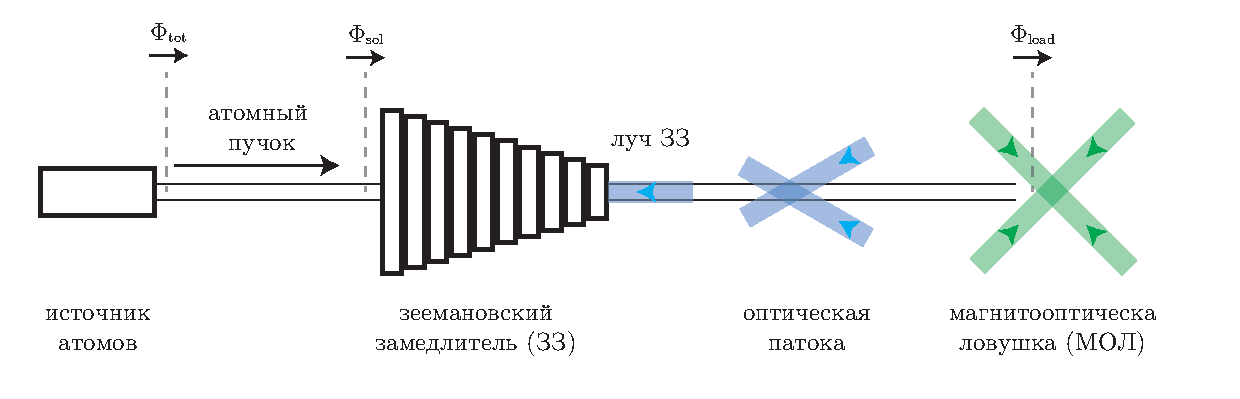
\includegraphics[width=1.0\textwidth]{figs/sheme.pdf}
    \caption{Принципиальная схема установки}
    %\label{fig:}
\end{figure}

Lorem ipsum dolor sit amet, consectetur adipisicing elit, sed do eiusmod
tempor incididunt ut labore et dolore magna aliqua. Ut enim ad minim veniam,
quis nostrud exercitation ullamco laboris nisi ut aliquip ex ea commodo
consequat. Duis aute irure dolor in reprehenderit in voluptate velit esse
cillum dolore eu fugiat nulla pariatur. Excepteur sint occaecat cupidatat non
proident, sunt in culpa qui officia deserunt mollit anim id est laborum.







%%%%%%%%%%%%%%%%%%%%%%%%%%%%%%%%%%%%%%%%%%%%%%%%%%%%%%%%%%%%%%%%%%%%%%%%%%%%%%%%
\unewpage
\section{Моделирование охлаждения атомов}
%%%%%%%%%%%%%%%%%%%%%%%%%%%%%%%%%%%%%%%%%%%%%%%%%%%%%%%%%%%%%%%%%%%%%%%%%%%%%%%%


\subsection{Печь}




\startp
\upar{Расход атомов}
В печи нагревается тулий до температуры $T$, вылетает из сопла диаметра $\sub{D}{ov}$, площади $\sub{S}{ov} = \pi \sub{D}{ov}^2/4$, длины $\sub{L}{ov}$. Полный поток атомов тулия \cite{tiecke_high-flux_2009} может быть определён, как 
\begin{equation}
	\sub{\Phi}{tot} = \frac{1}{4} \sub{n}{sat} \bar{v} \sub{S}{ov},
\end{equation}
где $\bar{v} = \sqrt{{8 \sub{k}{B} T}/{\pi m}}$ -- средняя тепловая скорость, $\sub{n}{sat} = \sub{P}{sat} / \sub{k}{B} T$ -- концентрация атомов в печи, зависимость $\sub{P}{sat} (T)$ для тулия приведена в \cite{alcock_vapour_1983} (точность в пределах $\pm 5\%$ в диапазоне 300-1400 К):
\begin{equation}
	\sub{P}{sat}(T) [\text{Па}] = 101325 \times 10^{
		8.882 - 12270\, T^{-1} - 0.9564 \log_{10} T
	}.
\end{equation}
Время работы печи тогда может найти, как $\sub{t}{life} = \sub{N}{tm} / \sub{\Phi}{tot}$.


\upar{Поток атомов на выходе}
В соответсвии с \cite{ramsey_molecular_1985}, вероятность вылететь из печи пропорциональна скорости $v$, поэтому максвелловское распределение модифицируется. 
Поток атомов со скоростью меньшей некоторой $\sub{v}{crit}$ на выходе из печи может быть найден \cite{tiecke_high-flux_2009}, как
\begin{equation}
	\sub{\Phi}{sol} = 
	\int_{0}^{\sub{\Omega}{sol}} d \Omega \frac{\cos \theta}{4\pi} \frac{1}{\mathcal N} 
	\int_{0}^{\sub{v}{crit}} v^3 e^{-(v/\alpha)^2} \d v \approx
	\frac{\sub{\Omega}{sol}}{4 \pi} \frac{1}{\mathcal N} 
	\int_{0}^{\sub{v}{crit}} v^3 e^{-(v/\alpha)^2} \d v
	,
\end{equation}
где $\alpha = \sqrt{2 \sub{k}{B} T/m}$ -- наиболее вероятная скорость, $\mathcal N = \int v^2 e^{-(v/\alpha)^2} \d v = \frac{\sqrt{\pi}}{4} \alpha^3$ -- нормирующий множитель распределения по скоростям. 


\upar{Распределение по скоростям}
Считая, что из печи вылетают только атомы с $v_r / v_z < \sub{\varphi}{ov} \approx \sub{D}{ov} / \sub{L}{ov}$, можем оценить распределение по $v_z$
\begin{equation}
	f(v_z) \propto \int_{0}^{\infty}  v_r e^{-(v_r/\alpha)^2} v_z e^{-(v_z/\alpha)^2} \theta(\sub{\varphi}{ov} - v_r/v_z) \d v_r \propto \frac{\sub{\varphi}{ov}^2}{\alpha^2} v_z^3 e^{-(v_z/\alpha)^2}.
\end{equation}
Аналогично можем посмотреть на распределение в радиальном направлении
\begin{equation}
	f(v_r) \propto \frac{2}{\alpha^2} \int_{0}^{\infty}  v_r e^{-(v_r/\alpha)^2} v_z e^{-(v_z/\alpha)^2} \theta(\sub{\varphi}{ov} - v_r/v_z) \d v_z \propto v_r e^{-(v_r/\alpha \sub{\varphi}{ov})^2}.
\end{equation}





\unewpage
\subsection{Зеемановский замедлитель} 
\startp
\upar{Магнитное поле} 
Для использующегося зеемановского замедлителя зависимость \cite{vlad} магнитного поля $\sub{B}{exp}$ от координаты $z$ представлена на рис. \ref{fig:zB}. В соответсвие с \cite{stack} магнитное поле эффективно замедляет атомы, при  $B(z) \propto \sqrt{1-z/z_0}$, на рисунке \ref{fig:zB} видно, что эта зависимость достаточно хорошо приближает $\sub{B}{exp}(z)$.
Параметры аппроксимации: $z_0 = \meas{94}{1}{см}$, $\delta z = \meas{15}{1}{см}$, $B_0 = \meas{740}{13}{Гс}$, $B_1 = \meas{260}{12}{см}$. 

\begin{figure}[ht]
    \centering
    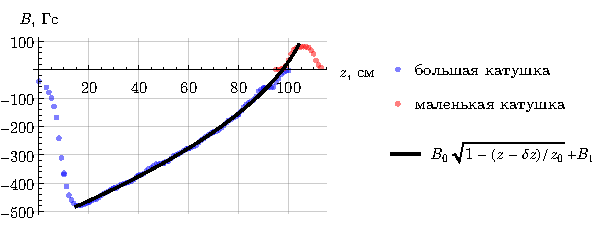
\includegraphics{figs/Bz.pdf}
    \caption{Зависимость магнитного поля внутри зеемановского замедлителя от координаты}
    \label{fig:zB}
\end{figure}

\upar{Тормозящая сила}
Считая, что мы работаем с циклическим переходом \red{(указать каким)}, в приближение двухуровневой системы, эффективное сила, действующая со стороны лазерного луча на атом, может быть записана в виде\footnote{
    Нагрев, связанный с изотропным излучением фотона, приводящий во время движения к случайным блужданиям в пространстве поперечных скоростей в данной работе не рассматривается, потери связанные с этим эффектом обычно ограничиваются 10\% \red{(добавить ссылку)}. 
}  \red{(добавить ссылку)}
\begin{equation}
    F = \frac{\hbar k \Gamma}{2} \frac{s}{1+s+4({\delta}+k v)^2/\Gamma^2}
\end{equation}
где $s=I/\sub{I}{sat}$ -- параметр насыщения, $\sub{I}{sat}$ -- интенсивность насыщения, $v$ -- скорость атома, $k$ -- волновой вектор. 

Уравнение движения запишется в виде
\begin{equation}
    \frac{d v}{d t} = \frac{F}{m},
    \hspace{0.25cm} \overset{v \d t = \d z}{\Leftrightarrow}  \hspace{0.25cm}
    \frac{d v(z)}{d z} = \frac{F(v, z)}{m \, v(z)},
\end{equation}
где $m$ -- масса атома. Таким образом можем найти зависимость $v(z)$ для различных $v_0 \overset{\mathrm{def}}{=} v(z=0)$, характерный вид приведен на рис. \ref{fig:vZz} для $\delta = -20\Gamma$, $s=20$, $B(z) \approx \sub{B}{exp}(z)$.
\begin{figure}[ht]
    \centering
    \subfigure[]{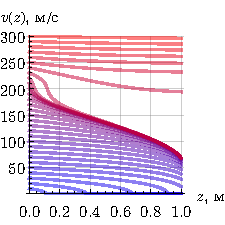
\includegraphics{figs/vz.pdf}}
    \hspace{10 mm} 
    \subfigure[]{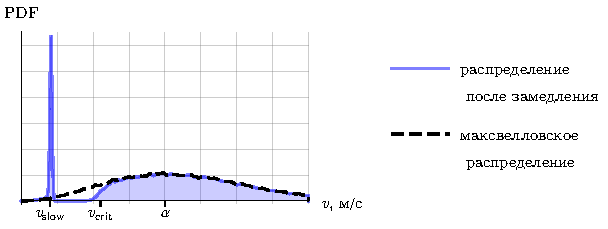
\includegraphics{figs/vdist_v2.pdf}}
    \vspace{-3mm}
    % zeeman_sim_v2
    \caption{a) Зависимость скорости атомов от координаты в зеемановском замедлителе. b) Характерное преобразование распределения атомов по скоростям после замедления}
    \label{fig:vZz}
\end{figure}

% заменить график на отнсительные величины

Для атомов со скоростями $v < \sub{v}{crit}$ замедлитель работает эффективно и замедляет до некоторой характерной $\sub{v}{slow}$, рядом с которой атомы распределены на масштабе \red{(добавить ссылку)} $\frac{1}{2}\Gamma\sqrt{1+s} / k$, характерное преобразование распределения\footnote{
    \textit{Забавный факт}. Впервые данный способ охлаждения атомов применялся \cite{__1981} для охлаждения Na до 1.5\,К в продольном направление  в 1981 году.
}  атомов по скоростям приведено на рис. \ref{fig:vZz}b, полученное в результате моделирования методом Монте-Карло для $10^5$ частиц. Обычно для зеемановского замедлителя выполняется, что $\sub{v}{crit} < \alpha$. 


% ~ 2 м/c * sqrt(1+s)


% \unewpage
\upar{Эффективность замедлителя}
Рассмотрим поток частиц, долетающих до замедлителя с учётом геометрии системы: $v_r/v_z < \sub{\varphi}{in} \sim 1/40$. Частицы распределены в соотвествии с \red{(добавить ссылку)}
\begin{equation}
    f(v_z, v_r) \propto v_r e^{-(v_r/\alpha)^2} v_z e^{-(v_z/\alpha)^2} \theta(\sub{\varphi}{in} - v_r/v_z).
    \label{ftheta}
\end{equation}
В дальнейшем в моделировании будет использоваться $10^6$ частиц из распределения \eqref{ftheta} для $\alpha = 300\un{м/c}$.

После замедлителя атомы попадают в магнитооптическую ловушку \red{(написать про патоку)}, основным параметром которой является скорость захвата $\sub{v}{cap}$ -- максимальная скорость атома, при которой атом захватывается ловушкой. 

\begin{figure}[ht]
    \centering
    \rotatebox{90}{\hspace{10mm}\scalebox{0.8}{$B_0=700\un{Гс}$ \hspace{22 mm} $B_0=500\un{Гс}$}}
    \hspace{2 mm} 
    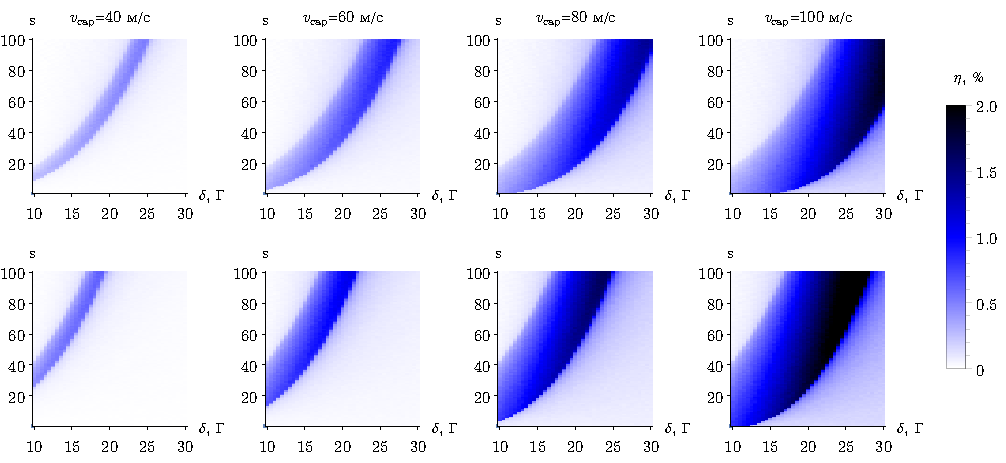
\includegraphics[width=0.95\textwidth]{figs/etas_v3.pdf}
    \caption{Эффективность работы замедлителя}
    \label{fig:eta}
\end{figure}

Для оценки эффективности системы замедлитель + МОЛ введём интегральный параметр $\eta$, равный отношению количества захваченных в МОЛ к количеству атомов, попадающих в замедлитель. Связь $\eta$ с наблюдаемым количеством атомов в МОЛ приведена в \eqref{eq:etaN}. 

Зависимость $\eta(B_0, \sub{v}{cap}, \delta, s)$ приведена на рисунке \ref{fig:eta}.  Моделирование методом Монте-Карло проводилось для $10^5$ частиц относящихся к распределению в потоке $\sub{\Phi}{sol}$. Учтены конечные размеры пространства внутри замедлителя (трубка радиуса порядка 1 см), влияние гравитации, конечные размеры МОЛ в соответсвии с характерными экспериментальными значениями установки.  
% нужно упомянуть влияние поперечного нагрева


\red{Здесь анализ картинки, мне не нравится -- переписать.}
Видно, что есть некоторая оптимальная область параметров (в которой $\sub{v}{slow} < \sub{v}{cap}$), ширина которой увеличивается с увеличением $\sub{v}{cap}$. Формально отстройкой $\delta$ и магнитным полем $B_0$ мы можем увеличивать $\sub{v}{crit}$ \red{(? добавить зависимость $\sub{v}{crit}(B_0, \delta)$, подумать про аналитические оценки)}, ценой увеличения $\sub{v}{slow}$. Увеличением мощности уменьшаем значение $\sub{v}{slow}$ до момента, когда $\sub{v}{slow} < \sub{v}{cap}$. Важно заметить, что зависимость $\eta$ от настраиваемых параметров носит унимодальный характер, что позволяет подбирать оптимальные значения итеративно находя максимум $\eta$ отдельно по каждому из параметров. 


% \phantom{42}

% \textbf{Экспериментальные данные}. \red{Снять зависимость $\NMOT(s)$ для разных магнитных полей.}


% \unewpage
% \subsection{Оптическая патока} 
% \input{parts/molases}


\unewpage
\subsection{Магнито-оптическая ловушка} \label{subsec:мол}
% 3.1. оптическая патока
% 3.2. мол
% 


\startp
\upar{Оптическая патока}
Рассмотрим подробнее принцип работы МОЛ в модели двухуровнего атома. Давление со стороны света на атомы формируется за счёт поглощения фотонов, которое зависит от отстройки $\delta$ от резонансной частоты перехода. Из-за эффекта Доплера, движущийся атом взаимодействует в его системе отсчета со света на сдвинутой частоте $- \frac{1}{2\pi} \vc{k} \cdot \vc{v}$, где $|\vc{k}| = \frac{2\pi}{c}\nu$, $c$ -- скорость света. Поглощая фотон атом получает импульс $\hbar \vc{k}$. Усредняя по большому числу актов поглощения и испускания, введем силу светового давления, определяющую изменения импульса атома $\vc{p}$. Учитывая изотропность спонтанного излучения, то есть отсутствие вклада в силу после усреднения по времени, в модели двухуровнего атома сила имеет вид
\begin{equation}
	\vc{F} = \langle \sub{n}{e} / \sub{n}{g} \rangle \cdot \hbar \vc{k} / \tau,
\end{equation}
где $\langle \sub{n}{e} / \sub{n}{g} \rangle$ -- доля возбужденных атомов, $\tau = 1/\Gamma$ -- время жизни возбужденного состояния, равная
\begin{equation}
	\left\langle 
		\frac{\sub{n}{e}}{\sub{n}{g}}
	\right\rangle = \frac{1}{2} \frac{s}{1+s+4\left(\frac{2 \pi \delta + \vc{k} \vc{v}}{\Gamma}\right)^2}.
\end{equation}
Заметим, что значение $s=1$ соответствует $\langle \sub{n}{e} / \sub{n}{g} \rangle=1/4$. Рассмотрим атом со скоростью $\vc{v}$, движение полностью определяется $\vc{F} \parallel \vc{v}$, c $\vc{k} \vc{v} = \pm k v$
\begin{equation}
	\vc{F} = \frac{\hbar \vc{k} \Gamma}{2}\left(
		\frac{s}{1+s+4\left(\frac{2\pi \delta - \vc{k} \vc{v}}{\Gamma}\right)^2}-
		\frac{s}{1+s+4\left(\frac{2\pi \delta + \vc{k} \vc{v}}{\Gamma}\right)^2}
	\right),
	\label{eq:FM1}
\end{equation}
а значит можем выразить силу в виде $\vc{F} = \alpha \vc{v}$:
\begin{equation}
	\vc{F} = \delta \frac{8 \hbar k^2  s / \Gamma}{
		\left(
			1+s+4\left(\frac{2\pi \delta - \vc{k} \vc{v}}{\Gamma}\right)^2
		\right)\left(
			1+s+4\left(\frac{2\pi\delta+\vc{k} \vc{v}}{\Gamma}\right)^2
		\right)
	}\vc{v},
	\label{eq:FM2}
\end{equation}
где $\Gamma$ -- естественная ширина линии. Для $\delta < 0$ (красной отстройки) получается вязкая среда, тормозящая атомы. 



\upar{Магнитооптическая ловушка}
Для локализации атомов в пространстве можно добавить в систему квадрупольное магнитное поле. Это легко сделать с помощью пары катушек в антигельмгольцевской конфигурации \cite{PhysRevA83}. Для пары колец магнитное поле вблизи центра может быть записано в виде
\begin{equation}
	\vc{B} = \beta (-x,\,  -y,\, 2z)\T/2,
	\hspace{10 mm} 
	\beta = \frac{3 \mu_0 I a R^2}{2(R^2+a^2)^{5/2}},
	\label{eq:B}
\end{equation}
где $I$ -- сила тока в катушках, $2a$ -- расстояние между катушками, $R$ -- радиус катушек, $\mu_0$ -- магнитная постоянная \cite{PhysRevA83}. Для катушек достаточно просуммировать магнитное поле от колец, прийдя к виду аналогичному \eqref{eq:B}. 

Рассмотрим переход $\ket{\text{g}} \to \ket{\text{e}}$ для $\sub{F}{g} = 4$ и $\sub{F}{e} = 5$. Для простоты будем считать только отклонения вдоль оси $z$. Из-за эффекта Зеемана уровни сдвинутся на величину $\Delta E = - \vc{B} \vc{\mu} = g_F m_F \subt{\mu}{B} \beta z$, где $g_F$ -- $g$-фактор Ланде, $m_F$ -- проекция магнитного момента на ось $z$, $\subt{\mu}{B}$ -- магнетон Бора. Аналогично вдоль других осей.

Поляризация света для каждого пучка патоки выбрана циркулярной и различной для пары \cite{vlad}, поэтому возможны переходы только с  $\Delta m_F = m_{\sub{F}{e}}-m_{\sub{F}{g}}= \pm 1$. Так как для используемого перехода на длине волны 530.7 нм $g \approx 1$, полный сдвиг по энергии может быть записан в виде $\Delta E_{\pm} \approx \pm \subt{\mu}{B} \beta z$, где знак определяется поляризацией. 

Подставляя сдвиг резонанса на величину $\Delta E_{\pm} / \hbar$ в \eqref{eq:FM1}, с учётом малости скоростей $k v < \Gamma$, близости к центру ловушки $\vc{r} \ll \sqrt{R a}$, можем линеаризовать выражение для силы $\vc{F}$:
\begin{equation}
	\vc{F}(\vc{r}, \vc{v}) = -\alpha \vc{v} - \varkappa \vc{r},
	\hspace{5 mm} 
	\varkappa = \frac{-\delta}{\Gamma/2\pi}\frac{8 \subt{\mu}{B} \beta k s}{\left(1+s+4\left(\frac{2\pi \delta}{\Gamma}\right)^2\right)^2},
	\hspace{5 mm} 
	\alpha = \frac{-\delta}{\Gamma} \frac{8 \hbar k^2 s}{\left(1+s+4\left(\frac{2\pi \delta}{\Gamma}\right)^2\right)^2},
\end{equation}
где $\vc{r}$  -- координаты атома.











% \unewpage
% \startp
\upar{Динамика количества атомов в МОЛ}
Количество атомов в ловушке $N$ во время загрузки может быть оценено уравнением \cite{vlad}
\begin{equation}
	\frac{d N}{d t} = \sub{\Phi}{load} - \gamma N - \tilde{\beta} \int_V n(\vc{r}, t)^2 \d^3 \vc{r},
\end{equation}
где $\gamma$ -- коэффициент линейных потерь, обусловленных столкновениями с буферным газом, $\beta$ -- скорость неэластичных бинарных столкновений, $n(\vc{r}, t)$ -- концентрация атомов, $V$ -- объем атомного облака, $\sub{\Phi}{load} = \eta \sub{\Phi}{sol}$ -- поток атомов после замедлителя со скоростью $v < \sub{v}{cap}$. Зависимость $n(\vc{r})$ в каждый момент времени может быть аппроксимирована гауссовой функцией с дисперсиями $(w_x, x_y, w_z)$, что позволяет явно посчитать интеграл:
\begin{equation}
	\frac{d N}{d t}  = \sub{\Phi}{load}  - \gamma N - \beta N^2,
	\hspace{10 mm} 
	\beta = \frac{\tilde{\beta}}{V} = \frac{\tilde{\beta}}{(2\pi)^{3/2}} \frac{1}{w_x w_y w_z} .
	\label{eq:mot1}
\end{equation}
Физический смысл $w_{x, y,z}$ -- радиус атомного облака по уровню $e^{-1}$.

Решая уравнение \eqref{eq:mot1}, можем найти зависимость $N(t)$:
\begin{equation}
	N(t) = \frac{\sub{\Phi}{load}}{\gamma} \left(
		\frac{1}{2} + \frac{\mu}{\th \mu \gamma t }
	\right)^{-1}
	,
	\hspace{10 mm} 
	\mu \overset{\mathrm{def}}{=}  \frac{1}{2} \sqrt{1 + 4 \frac{\beta \sub{\Phi}{load}}{\gamma^2}}.
\end{equation}
Для достаточно большого времени загрузки $\gamma\, \mu\,  \sub{t}{load} \gg 1$ можем рассматривать стационарное значение и выразить связь $N$ с $\eta$:
\begin{equation}
	N = \frac{\gamma}{2\beta}
	\left(\sqrt{1 + 4 \frac{\beta \eta \Phi}{\gamma^2}}-1\right),
	\hspace{10mm} 
	\eta = \frac{\gamma}{\sub{\Phi}{sol}} N + \frac{\beta^2}{\sub{\Phi}{sol}} N^2.
	\label{eq:etaN}
\end{equation}
Таким образом задача оптимизации количества атомов в магнитооптической ловушке может быть сведено к оптимизации безразмерного параметра $\eta$.  


В эксперименте характерные значения \cite{vlad} $\gamma = 0.12\,\text{c}^{-1}$, $\tilde{\beta}=2\times10^{-10}\,\text{см}^{-3}/\text{c}$, $V=40\times 10^{-5}\, \text{см}^{-3}/\text{с}$, $\beta = 5\times 10^{-7}\,\text{c}^{-1}$, $\sub{\Phi}{load} \sim 10^8\,\text{c}^{-1}$. Так как $\beta \Phi \gg \gamma^2$, то с хорошей точностью можно считать $\gamma=0$, тогда уравнения существенно упрощаются:
\begin{equation}
	N(t) = \sqrt{\frac{\sub{\Phi}{load}}{\beta}} \left(1-e^{-t \sqrt{\beta \sub{\Phi}{load}}}\right) \overset{t\to\infty}{=} \sqrt{\frac{\sub{\Phi}{sol}}{\beta}\eta}.
	\label{eq:Ntd}
\end{equation}



\unewpage
\subsection{Двухмерная магнито-оптическая ловушка} 
% тут общее описание 2D-МОЛ





\startp
\upar{Поток загрузки}
В соответствии с формулой \eqref{oven}, а также считая, что захватываются все атомы со скоростью $v < \vcap$ \cite{hf}
\begin{equation}
	\sub{\Phi}{2d} \propto \sub{\Phi}{tot} \int_{0}^{\vcap} v^3 e^{-v^2/\alpha^2} \d v,
	\hspace{5 mm} 
	\sub{\Phi}{sol} = \sub{n}{sat} \bar{v} \sub{S}{ov} \frac{\sub{\Omega}{2d}}{4 \pi},
	\hspace{0.5cm} \Rightarrow \hspace{0.5cm}
	\sub{\Phi}{2d} \approx \frac{1}{2} \sub{\Phi}{sol} \left(\frac{\vcap}{\alpha}\right)^4,
	\label{eq:2dmotM}
\end{equation}
где $\sub{\Omega}{2d}$ -- телесный угол двухмерной магнитооптической ловушки. Таким образом основным параметром, определяющим поток атомов из 2D-МОЛ является скорость захвата.  Если сравнивать 2D-МОЛ с ЗЗ, то из \eqref{eq:eta} и \eqref{eq:2dmotM}, считая что почти все атомы из 2D-МОЛ попадают в МОЛ \cite{ravenhall_high-flux_2021}: $\sub{\eta}{2d} \sim \frac{1}{2}(\sub{v}{cap} / \alpha)^4$. Ожидаемая величина для нашей установки 



\upar{Скорость захвата} 
Тормозящая сила в МОЛ \cite[(3.1.5)]{vlad} может быть записана в виде
\begin{equation}
	F(v) = \frac{8 \hbar \delta k^2}{\Gamma} \frac{s}{\left(1+s+\left(\frac{\delta-kv}{\Gamma/2}\right)^2\right)\left(1+s+\left(\frac{\delta+kv}{\Gamma/2}\right)^2\right)}v.
	\label{eq:force2}
\end{equation}
Далее полагая $\d l = v \d t$, можем записать
\begin{equation}
	m \frac{dv}{dt} = F(v),
	\hspace{0.5cm} \Rightarrow \hspace{0.5cm}
	m \int_{\vcap}^{0} \frac{v}{F(v)} \d v = D,
	\label{eq:2dMOT}
\end{equation}
где $D$ -- диаметр лазерного пучка. В левой части получается полином пятой степени по $\vcap$. Полагая мощность лазера фиксированной  $P \sim 0.1$ Вт, можем выразить $s(D) = \frac{1}{\sub{I}{sat}}\frac{P}{\pi D^2/4}$.  Уравнение \eqref{eq:2dMOT} неявно задаёт зависимость $\vcap(\delta, s, D)$. Численным решением уравнения \eqref{eq:2dMOT}, найдены зависимости $\vcap(\delta, s, D)$, рис. \ref{fig:vcapDs}. 
Для наглядности представлены зависимости $\vcap(\delta, P, D=\text{5 мм})$: рис. \ref{fig:vcapflat}a, и $\vcap(\delta, P=\text{25 мВт}, D)$: рис. \ref{fig:vcapflat}б.


\begin{figure}[ht]
    \centering
    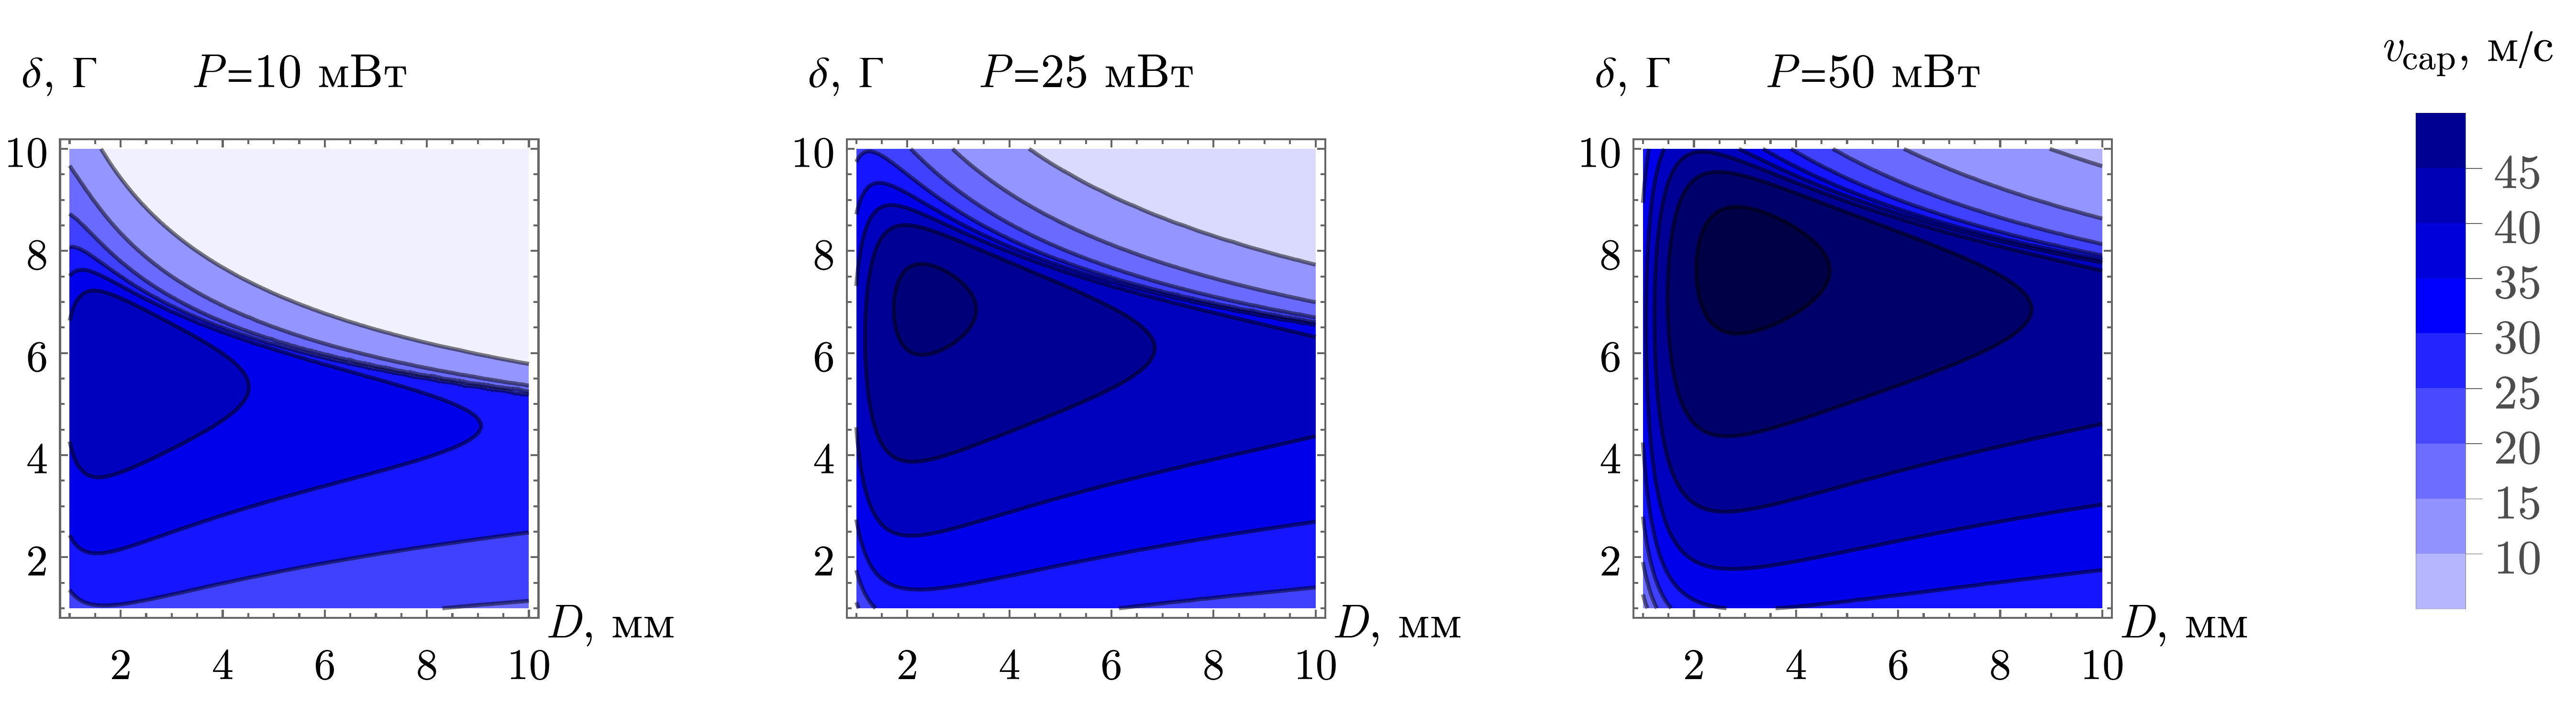
\includegraphics[width=1.0\textwidth]{figs/vcap2d_delta-Ds.png}
    \caption{Зависимость скорости захвата 2D-МОЛ для различных мощностей}
    \label{fig:vcapDs}
\end{figure}



\begin{figure}[ht]
    \centering
    \subfigure[]{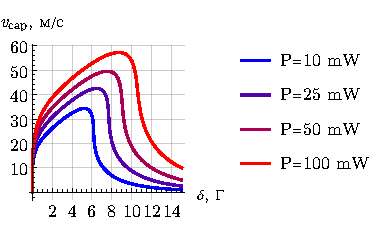
\includegraphics{figs/vcap2D_P.pdf}} %D=5мм
    \hspace{10 mm} 
    \subfigure[]{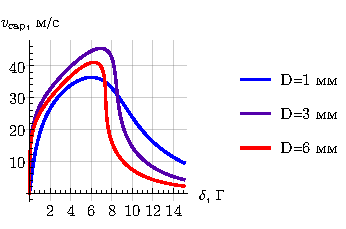
\includegraphics{figs/vcap2D_D.pdf}} %P=25мВт
    \vspace{-3mm}
    \caption{Зависимость скорости захвата от отстройки 
    и a) мощности при $D=5$ мм; б) размеров луча при $P = 25$ мВт.
    }
    \label{fig:vcapflat}
\end{figure}


\upar{Толкающий луч}
Из геометрии системы $v_r / v_y < \theta$, при этом $v_y < \vcap$, что приводит к $v_r < \theta \vcap \sim 1$ м/c. Под действием гравитации атомы могут просто не долетать до основной МОЛ, поэтому добавляется толкающий луч. 

Силу от одного толкающего луча можем найти в виде
\begin{equation}
	a(v) = F(v)/m = \frac{\hbar k}{m} \frac{\Gamma}{2} \frac{s}{1+s+\frac{(2 \pi \delta - k v)^2}{\Gamma^2/4}},
	\label{eq:force1}
\end{equation}
где для простоты считали $\delta = 0$. Также будем считать, что $\sub{v}{нач} = 0$, интересно найти зависимость $\sub{v}{кон}(s)$ при фиксированной величине длины разгона $l$:
\begin{equation}
	\int_{0}^{\sub{v}{кон}} \frac{v \d v}{a(v)} = \int_{0}^{l} \d l.
\end{equation}
Считая $s \gg \frac{\Gamma  m}{8 k^3 l \hbar } \sim 10^{-4}$, можем написать
\begin{equation}
	\sub{v}{кон}(l) = \left(\frac{\hbar \Gamma^3}{2 k m} ls\right)^{1/4}.
\end{equation}
Для $l\sim 20\,$см можем считать $\sub{v}{кон} \sim s^{1/4} \cdot 30\,\text{м/с}$.



Аналогично можем найти связь
\begin{equation}
		\int_{0}^{\sub{v}{кон}} \frac{\d v}{a(v)} = \int_{0}^{t} \d t,
		\hspace{0.5cm} \Rightarrow \hspace{0.5cm}
		\sub{v}{кон}(t) = \frac{\Gamma}{2}  \left(\frac{3 s t \hbar }{k m}\right)^{1/3}.
\end{equation}
Теперь можем записать связь на время и на критическую длину:
\begin{equation}
	t = \frac{2^{9/4}}{3} \left(\frac{k m}{s \Gamma^3 \hbar}\right)^{1/4} l^{3/4} = \frac{4}{3} \frac{l}{\sub{v}{кон}},
	\hspace{10 mm} 
	\sub{l}{крит} \sim 
	% \frac{3}{2^{3/2}} 
	\sqrt{\frac{\sub{h}{крит} \sub{v}{cap}^2}{g}},
	 % \approx 0.03 \frac{l^{3/4}}{s^{1/4}}.
\end{equation}
где $\sub{h}{крит}$ определяется геометрией вакуумной установки.




% \unewpage
% \upar{Усиленные встречные пучки}
% Так как основные требования к $\vcap$ возникают в торможение летящих из печки атомов, то имеет смысл перераспределить мощность в пучках 2D-МОЛ так, чтобы во встречных пучках было больше мощности. Данный приём аналогичен расположению двухмерной оптической патоки перед МОЛ. Подобные конфигурации обычно называются 2D${}^+$МОЛ. На рис. \ref{fig:motplus} приведена оценка $\sub{v}{cap}$ для фиксированной мощности $P=25\,$мВт. 

% % Совмещая \eqref{eq:force1} и \eqref{eq:force2}, находим тормозящую силу \red{(не дописано)}
% % \begin{equation*}
	
% % \end{equation*}
% % где $\alpha P$ мощности уходит на дополнительную патоку, а $(1-\alpha)P$ участвует в 

% \begin{figure}[ht]
%     \centering
%     \subfigure[]{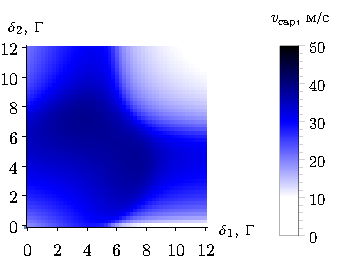
\includegraphics{figs/motplus1.pdf}}
%     \hspace{20 mm} 
%     \subfigure[]{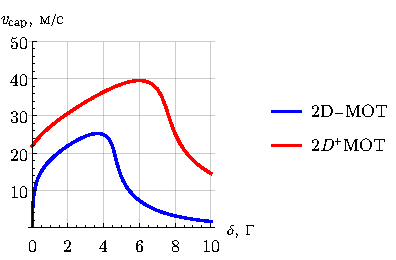
\includegraphics{figs/motplus2.pdf}} %5мм, 25 мВт
%     \vspace{-3mm}
%     % zeeman_sim_v2
%     \caption{a) Зависимость скорость захвата $\sub{v}{cap}$ для 2D-МОЛ от величины отстройки основной 2D-МОЛ $\delta_1$ и добавочных к встречным пучкам $\delta_2$. Видно, что можно использовать в качетстве добавки лучи той же частоты, что и основной 2D-МОЛ. б) Зависимость скорости захвата 2D-МОЛ от отстройки лучей 2D-МОЛ при $\delta=\delta_1=\delta_2$}
%     \label{fig:motplus}
% \end{figure}












%%%%%%%%%%%%%%%%%%%%%%%%%%%%%%%%%%%%%%%%%%%%%%%%%%%%%%%%%%%%%%%%%%%%%%%%%%%%%%%%
\unewpage
\section{Экспериментальные результаты}
%%%%%%%%%%%%%%%%%%%%%%%%%%%%%%%%%%%%%%%%%%%%%%%%%%%%%%%%%%%%%%%%%%%%%%%%%%%%%%%%

Откалибровано абсолютное значение температуры используемой печи. Описана схема детектирования атомов в МОЛ, описан алгоритм обработки фотографии и определения температуры облака атомов $T$ и полного количества атомов $N$. Снята зависимость $N$ от отстройки лучей МОЛ, токов ЗЗ и отстройки лучей ОП. Определены оптимальные значения, соответсвующие $\subt{\delta}{ОП} = -1.7\Gamma$, $\subt{\delta}{МОЛ} = -13.5\Gamma$ и $\sub{I}{small} = 18\,$А, $\sub{I}{big} = 35\,$А. Найденные значения соответсвуют температуре печи $T_2 = 680 \dC$ и $\sub{\Phi}{sol}(T_2) \sim 1 \times 10^{11}\,\text{c}^{-1}$. Раннее наша установка работала при температуре $T_1 = 730 \dC$, что соответсвует потоку атомов $\sub{\Phi}{sol}(T_1) \sim 5 \times 10^{11}\,\text{c}^{-1}$. Таким образом время работы установки было увеличено в 5 раз до 5 месяцев непрерывной работы, при этом поток загрузки МОЛ $\sub{\Phi}{load} \sim 10^8$ остался на том же уровне.









%%%%%%%%%%%%%%%%%%%%%%%%%%%%%%%%%%%%%%%%%%%%%%%%%%%%%%%%%%%%%%%%%%%%%%%%%%%%%%%%
\unewpage
\section{Заключение}
%%%%%%%%%%%%%%%%%%%%%%%%%%%%%%%%%%%%%%%%%%%%%%%%%%%%%%%%%%%%%%%%%%%%%%%%%%%%%%%%




\unewpage
\addcontentsline{toc}{section}{Список литературы}
\bibliography{bib}



% --------------------- для заметок -----------------------------
% добавить описание замедлителя
% описание МОЛ
% вычисление $\sub{v}{cap}$
% патока, вклад в $\sub{v}{cap}$
% Добавить раздел с калибровкой печи?
% 